% Created 2018-11-14 Wed 12:21
% Intended LaTeX compiler: pdflatex
\documentclass[11pt]{article}
\usepackage[utf8]{inputenc}
\usepackage[T1]{fontenc}
\usepackage{graphicx}
\usepackage{grffile}
\usepackage{longtable}
\usepackage{wrapfig}
\usepackage{rotating}
\usepackage[normalem]{ulem}
\usepackage{amsmath}
\usepackage{textcomp}
\usepackage{amssymb}
\usepackage{capt-of}
\usepackage{hyperref}
\usepackage{minted}
\usepackage{sectsty}
\allsectionsfont{\sffamily}
\usepackage{amssymb}
\usepackage[normalem]{ulem}
\renewcommand{\d}{\ensuremath{\mathrm{d}}}
\setlength{\textheight}{21cm}
\setlength{\textwidth}{16cm}
\setlength{\evensidemargin}{-0cm}
\setlength{\oddsidemargin}{-0cm}
\setlength{\topmargin}{0cm}
\renewcommand{\baselinestretch}{1.2}
%\renewcommand{\topfraction}{0.8}
%\renewcommand{\bottomfraction}{0.6}
%\renewcommand{\textfraction}{0.2}
\date{}
\title{}
\hypersetup{
 pdfauthor={Dinesh A},
 pdftitle={},
 pdfkeywords={},
 pdfsubject={},
 pdfcreator={Emacs 25.1.1 (Org mode 9.1.2)},
 pdflang={English}}
\begin{document}

\title{\sffamily \textbf{DEM Physics and its implementation}}

\author{Dinesh A, IIT Bombay}

\maketitle


\begin{abstract}
  Discrete element method explanation and implementation. This report mainly
  deals with RK2 implementation of DEM step.
\end{abstract}

\section{Post step equation description}
\label{sec:orge4d9814}
Let us say that we have five particles in our world which are contained in a
particle array named \emph{soil}. Say at time \(t=t0\) the particles are in a configuration of
figure \ref{fig:pars_t0}

\begin{figure}[H]
\centering
\includegraphics[scale=0.15]{dem_physics_figures/pars_t0.eps}
\caption{Particles at t0\label{fig:pars_t0}}
\end{figure}

The contact at time \(t0\) of particle 1 are

\begin{minted}[]{python}
       trk_idxs = [2, 3, 5, -1, -1, -1]
\end{minted}

After moving to the next time step by using our favorite integrator, the particles
at time \(t0+dt\) look like in figure \ref{fig:pars_t0_dt}

\begin{figure}[H]
\centering
\includegraphics[scale=0.25]{dem_physics_figures/pars_t0_dt.eps}
\caption{Particles at time t0+dt\label{fig:pars_t0_dt}}
\end{figure}

Now before we move on to start the computation at \(t0+dt\), we will update the
contact information of all the particles in our \emph{soil} by running an equation
in poststep.

After post step the \textbf{trk\_idxs}  are

\begin{minted}[]{python}
       trk_idxs = [2, 3, -1, -1, -1, -1]
\end{minted}

Well, \textbf{but} the actual contacts of particle 1 are 2, 3, 4. A point to be
noted, after the time step, we will only update the existing contact
information, we will not add any new contacts but will remove if any particle
left the contact. By moving from time \(t0\) to \(t0+dt\), particle 1
lost contact with particle 5, so we just updated that information.

\textbf{Note} that new contacts to a particle are added at the beginning of the time
step.  This update simplifies RK2 implementation. Let us see how.


\section{RK2 implementation in PySPH}
\label{sec:org8a9a5bb}
Let us start our system from the previous section. We are interested in the
dynamcis of the particle 1 which is in contact with
particles 2, 3, 4 at \(t0\). Since particle 4 came in to contact at time \(t0\), we don't
have it in out tracking list. Let's see how the tracking indices of particle 1
look, before we start the force and other computations.As expected particle 4
is not there in the list.

\begin{minted}[]{python}
       trk_idxs = [2, 3, -1, -1, -1, -1]
\end{minted}

RK2 integration scheme is implemented by \emph{EPECIntegrator} in PySPH which can
be found \href{https://github.com/pypr/pysph/blob/master/pysph/sph/integrator.py\#L249}{here}.

\begin{minted}[]{python}
	def one_timestep(self, t, dt):
	    self.initialize()

	    self.compute_accelerations()

	    # Predict
	    self.stage1()

	    # Call any post-stage functions.
	    self.do_post_stage(0.5*dt, 1)

	    self.compute_accelerations()

	    # Correct
	    self.stage2()

	    # Call any post-stage functions.
	    self.do_post_stage(dt, 2)
\end{minted}


In RK2, first we save the properties at time \(t0\) which can be used to move to
\(t0+dt\) by accelerations at time \(t0+dt/2\). Here we only focus on tangential
contact implementation. So at the beginning of the time step, the contact
information of particle 1 is,

\begin{minted}[]{python}
       trk_idxs = [2, 3, -1, -1, -1, -1]
\end{minted}

\noindent remember that the actual number of contacts particle 1 is actually
2, 3, 4. But from the previous time step we are only given 2, 3 as
contacts. The new particle 4 will be added while computing the forces (How?
This will elaborated).

In PySPH we save the particle properties in \emph{initialize} method. Let's save the
tangential overlap \emph{tng\_x} which is at time \(t0\) to \emph{tng\_x0}

\begin{minted}[]{python}
	def initialize(self, ...):
	    d_tng_x0[d_idx] = d_tng_x[d_idx]
\end{minted}

We will not save the tracking indices at time \(t0\).

After running \emph{initialize} the tangential overlap array looks like

\begin{minted}[]{python}
	def initialize(self, ...):
	    d_tng_x0[d_idx] = d_tng_x[d_idx]
	tng_x = [1.2, 2.1, 0., 0., 0.]
	tng_x0 = [1.2, 2.1, 0., 0., 0.]
	atang_x = [0.3, 0.2, 0., 0., 0.]
\end{minted}


Rest of the methods in integrator will be discussed using three use cases.

\begin{enumerate}
\item How would we deal with new contacts at time \(t0\)? Particle 4 comes under that case.
\item How would we deal with Particles leaving at half a time step? An example
will be given in its section.
\item What if a particle comes into contact at half time step? An example will be
given in its section.
\end{enumerate}

Before we begin let me remind you once again that \emph{tng\_x} and \emph{tng\_x0} are at time \(t0\).



\subsection{Case 1}
\label{sec:orgd62f31e}
\begin{figure}[H]
\centering
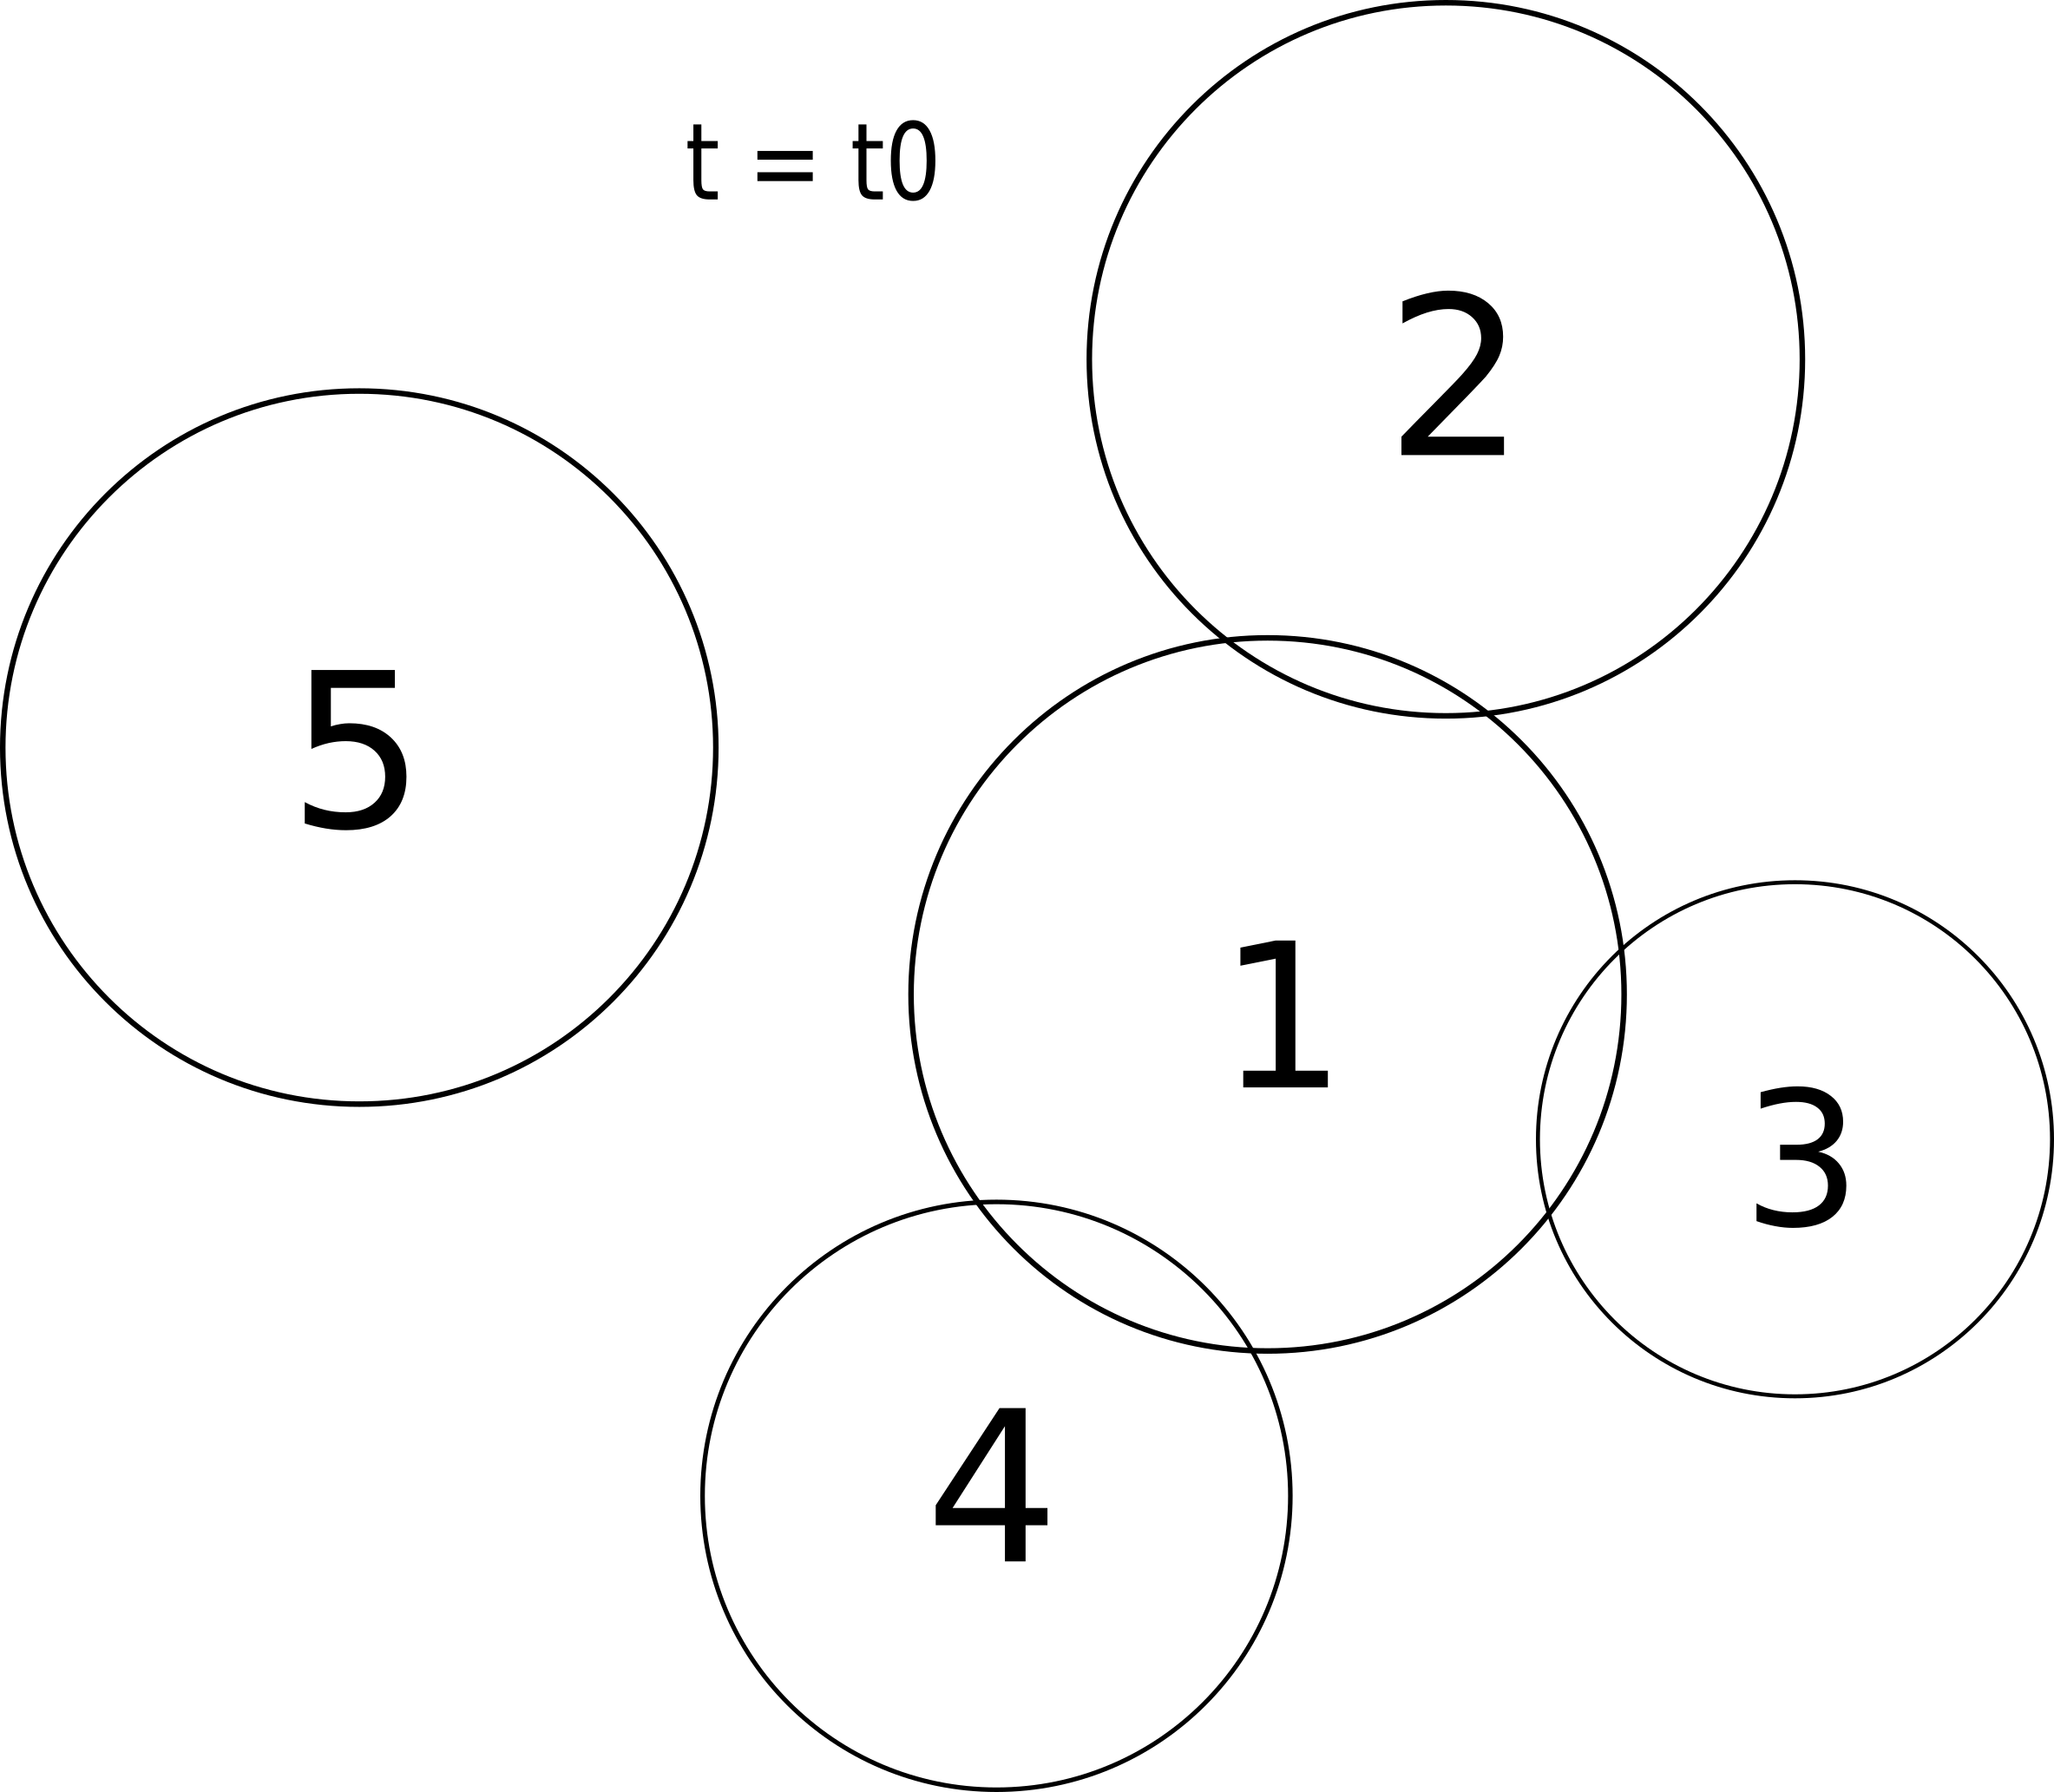
\includegraphics[scale=0.30]{dem_physics_figures/case1_t0.png}
\caption{Particles at time t0\label{fig:case1_t0}}
\end{figure}

This the present case. While computing the force, we will add the particle index
and tangential acceleration to \emph{atng\_x} and we won't touch \emph{tng\_x0}. And also increment
the count of total number of contacts.

\begin{minted}[]{python}
	 if found == 0:
	     found_at = q
	     d_tang_idx[found_at] = s_idx
	     d_total_tang_contacts[d_idx * d_total_dem_entities[0] +
				     s_dem_id[0]] += 1

	     # set the acceleration for the current time step
	     d_atang_x[found_at] = vt_x
\end{minted}


Here we should add particle 4 and also set its acceleration. After \emph{compute\_forces},
the tangential variables of particle 1 look like

\begin{minted}[]{python}
	tng_x0 = [1.2, 2.1, 0., 0., 0.]
	tng_x = [1.2, 2.1, 0., 0., 0.]
	trk_idxs = [2, 3, 4, -1, -1]
	atng_x = [1.2, 2.1, 1.4., 0.]
\end{minted}

In \emph{stage\_1} particles will move to half a time step, tangential overlap will
also be at \$t0+dt/2.\$.


\begin{minted}[]{python}
	def stage1(self, ...):
	    # Code elided. Only tangential update is given
	    for i in range(0, num_ctcs):
		d_tng_x[i] = d_tng_x0[i] + dtb2 * d_vt[i]
\end{minted}

Particle 1 tangential variables after stage 1 will look like,

\begin{minted}[]{python}
	tng_x0 = [1.2, 2.1, 0., 0., 0.]
	tng_x = [1.5, 3.1, 1.9, 0., 0.]
	trk_idxs = [2, 3, 4, -1, -1]
	atng_x = [1.2, 2.1, 1.4., 0.]
\end{minted}

Please note that the tangential displacement of particle 4 has some
value. Let us have a keen look at contact between 1 and 4. At the beginning
of the time step, we don't have the information of particle 4 to be in
contact with 1. While computing forces we added that to end of the tracking
indices. One assumption we made here is when the particle comes into contact
for a first time its tangential overlap will be zero. In our example particle
4 was newly added at time \(t0\). Which implies that its tangential
displacement at time \(t0\) is zero. Fortunately that is what \emph{tang\_x0} is
representing.

Now we \emph{compute\_accelerations} using the positions of particles at time
\(t0+dt/2\) and corresponding tangential displacements which are also
at time \(t0+dt/2\).

Finally in stage 2, using the accelerations at time \(t0+dt/2\) and positions
at time \(t0\) we progress the system to time \(t0+dt\). That would be

\begin{minted}[]{python}
	def stage2(self, ...):
	    # Code elided. Only tangential update is given
	    for i in range(0, num_ctcs):
		d_tng_x[i] = d_tng_x0[i] + dt * d_vt[i]
\end{minted}

This is will not create any problem with particle 4. Since we have

\begin{minted}[]{python}
	# Since particle 4 is at position 2
	d_tng_x[2] = d_tng_x0[2] + dt * d_vt[2]
\end{minted}

We are incrementing the tangential overlap of particle 4 which has zero
tangential overlap at time \(t0\) by using the acceleration at time \(t0+dt/2\),
which also satisfies the integration property.

Then final configuration of the particles may look like figure \ref{fig:case1_t0_dt}

\begin{figure}[H]
\centering
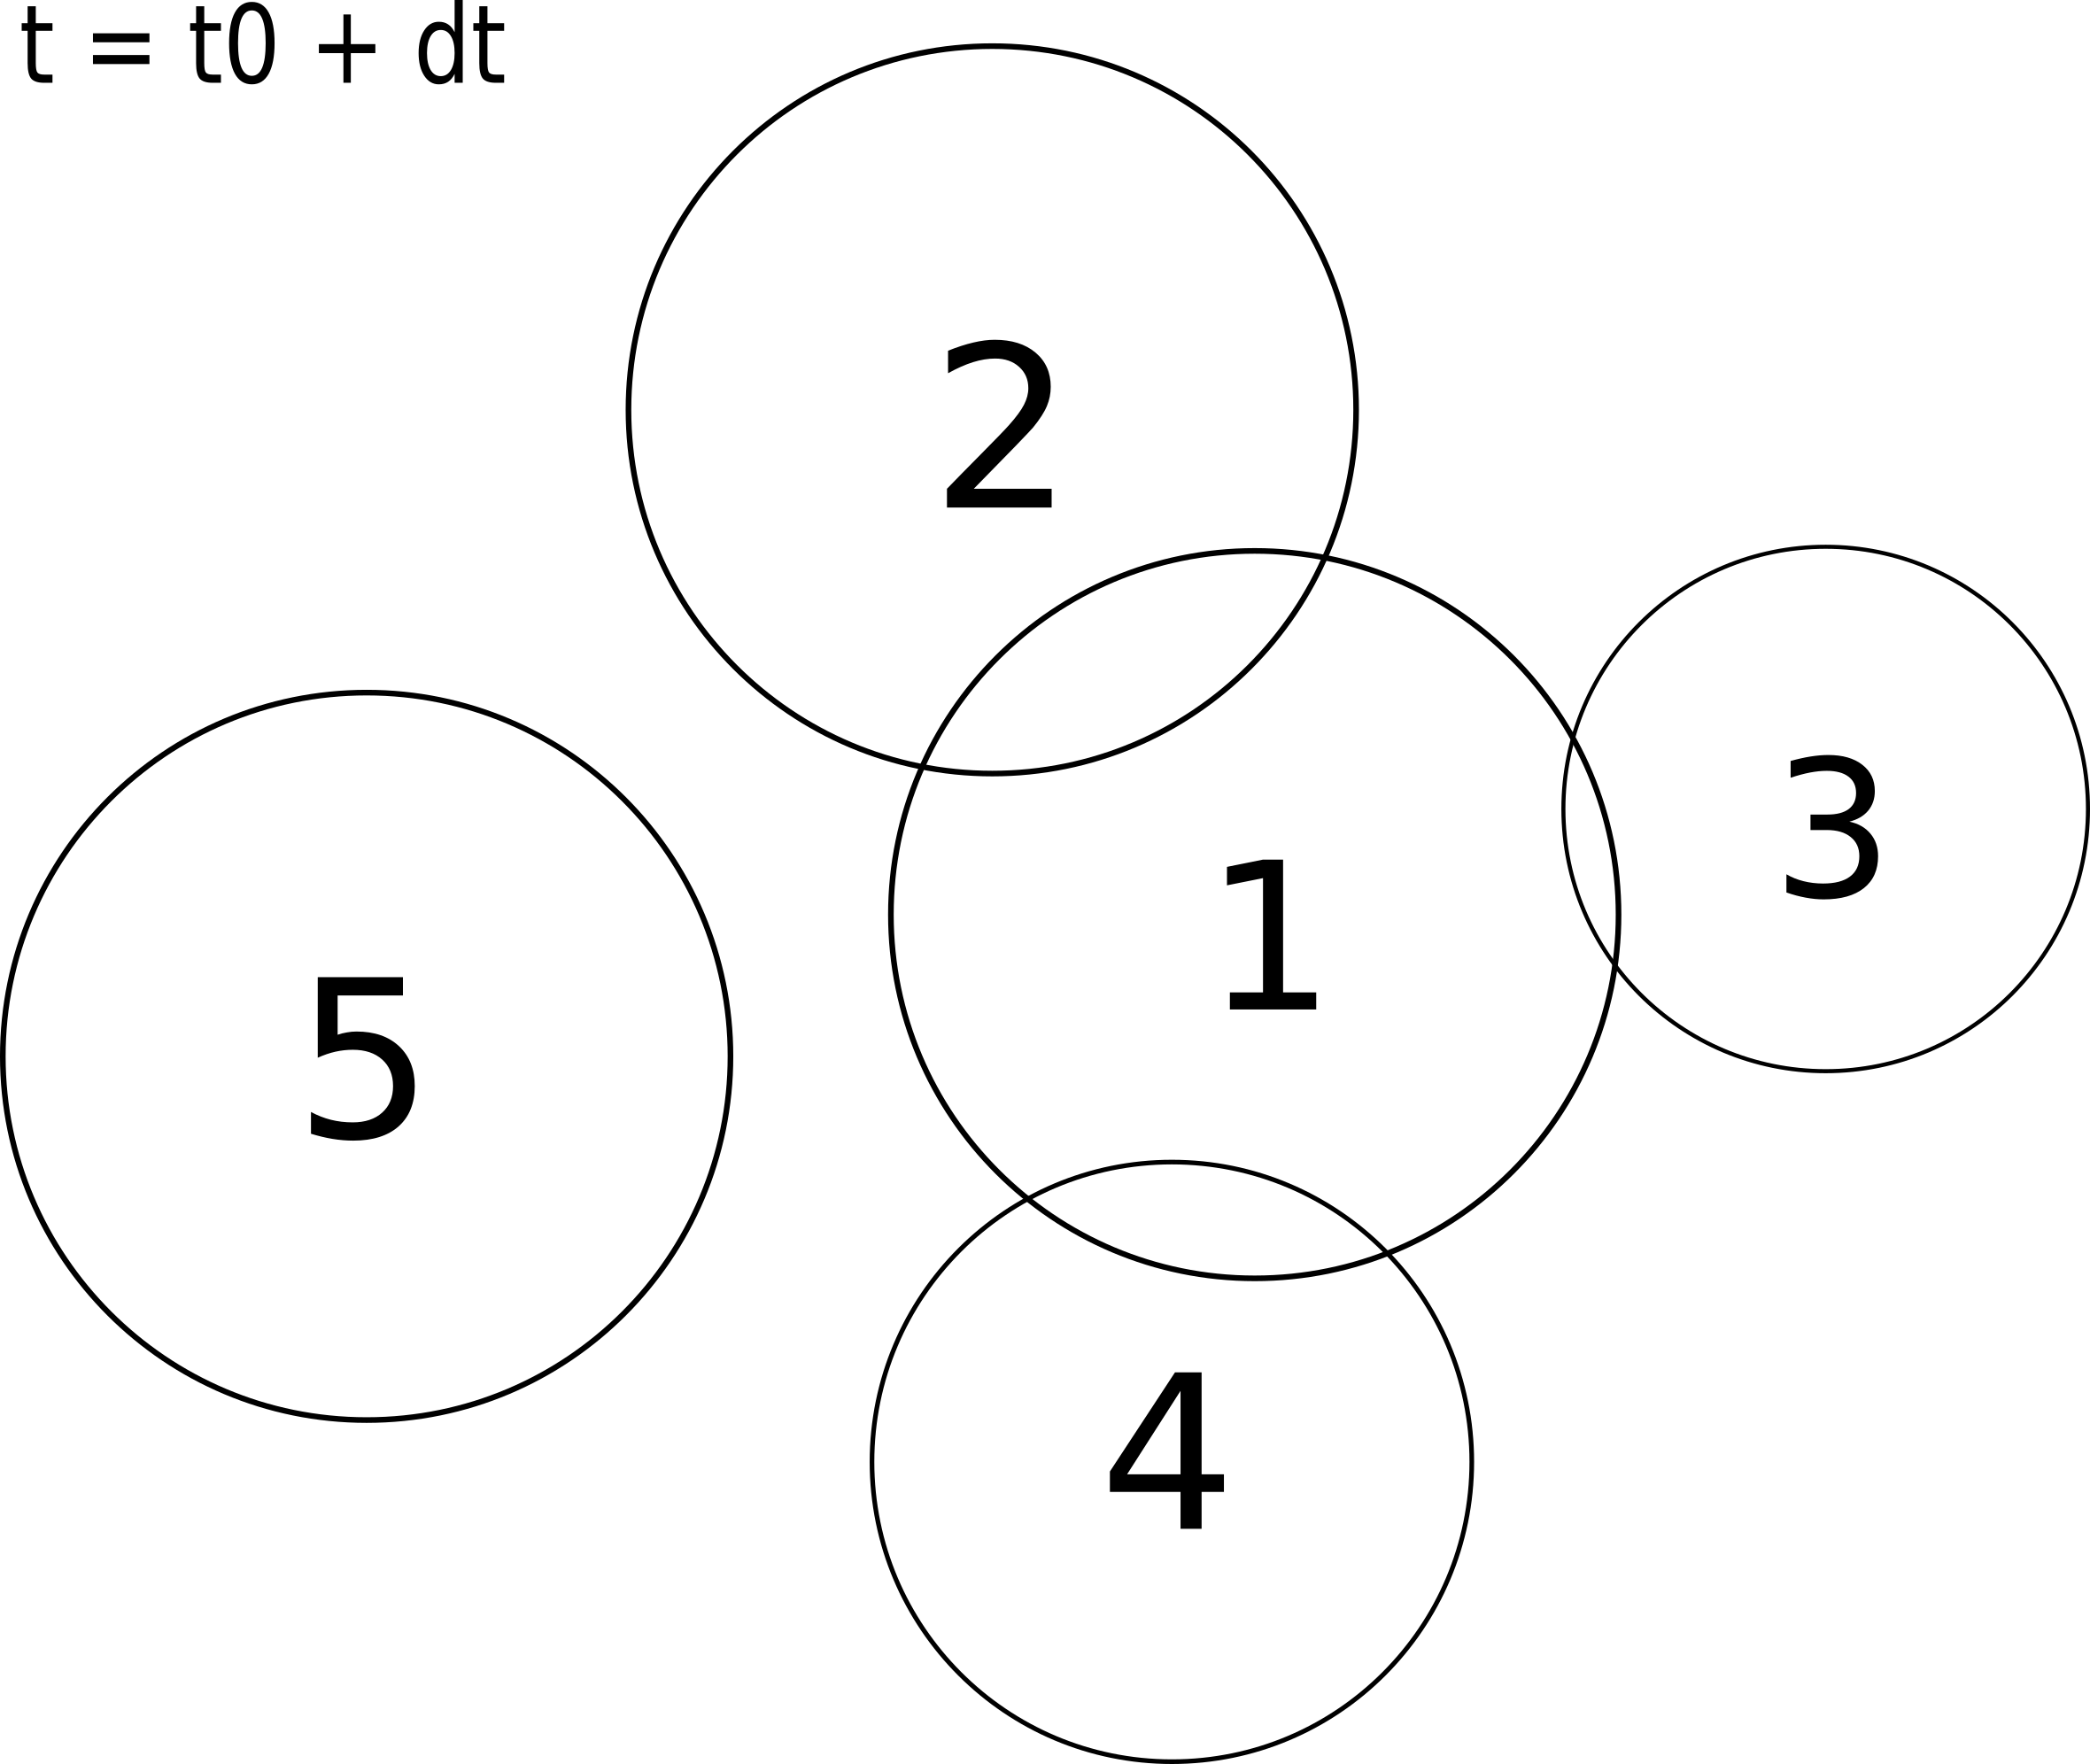
\includegraphics[scale=0.30]{dem_physics_figures/case1_t0_dt.png}
\caption{Particles at time t0 + dt\label{fig:case1_t0_dt}}
\end{figure}

Note: Updating the contact information after the time step is helpful here.

\subsection{Case 2}
\label{sec:org8bc9c9f}
In case 2 we deal with particle loosing contact at time \(t0 + dt/2\). For an
example take three particles 1, 2, 3. Say at time \(t0\) particle 2 and 3 are
in contact with particle 1. At time \(t0+dt/2\) particle 3 leaves contact with particle 1.
This is depicted in figure \ref{fig:case2}

\begin{figure}[H]
\centering
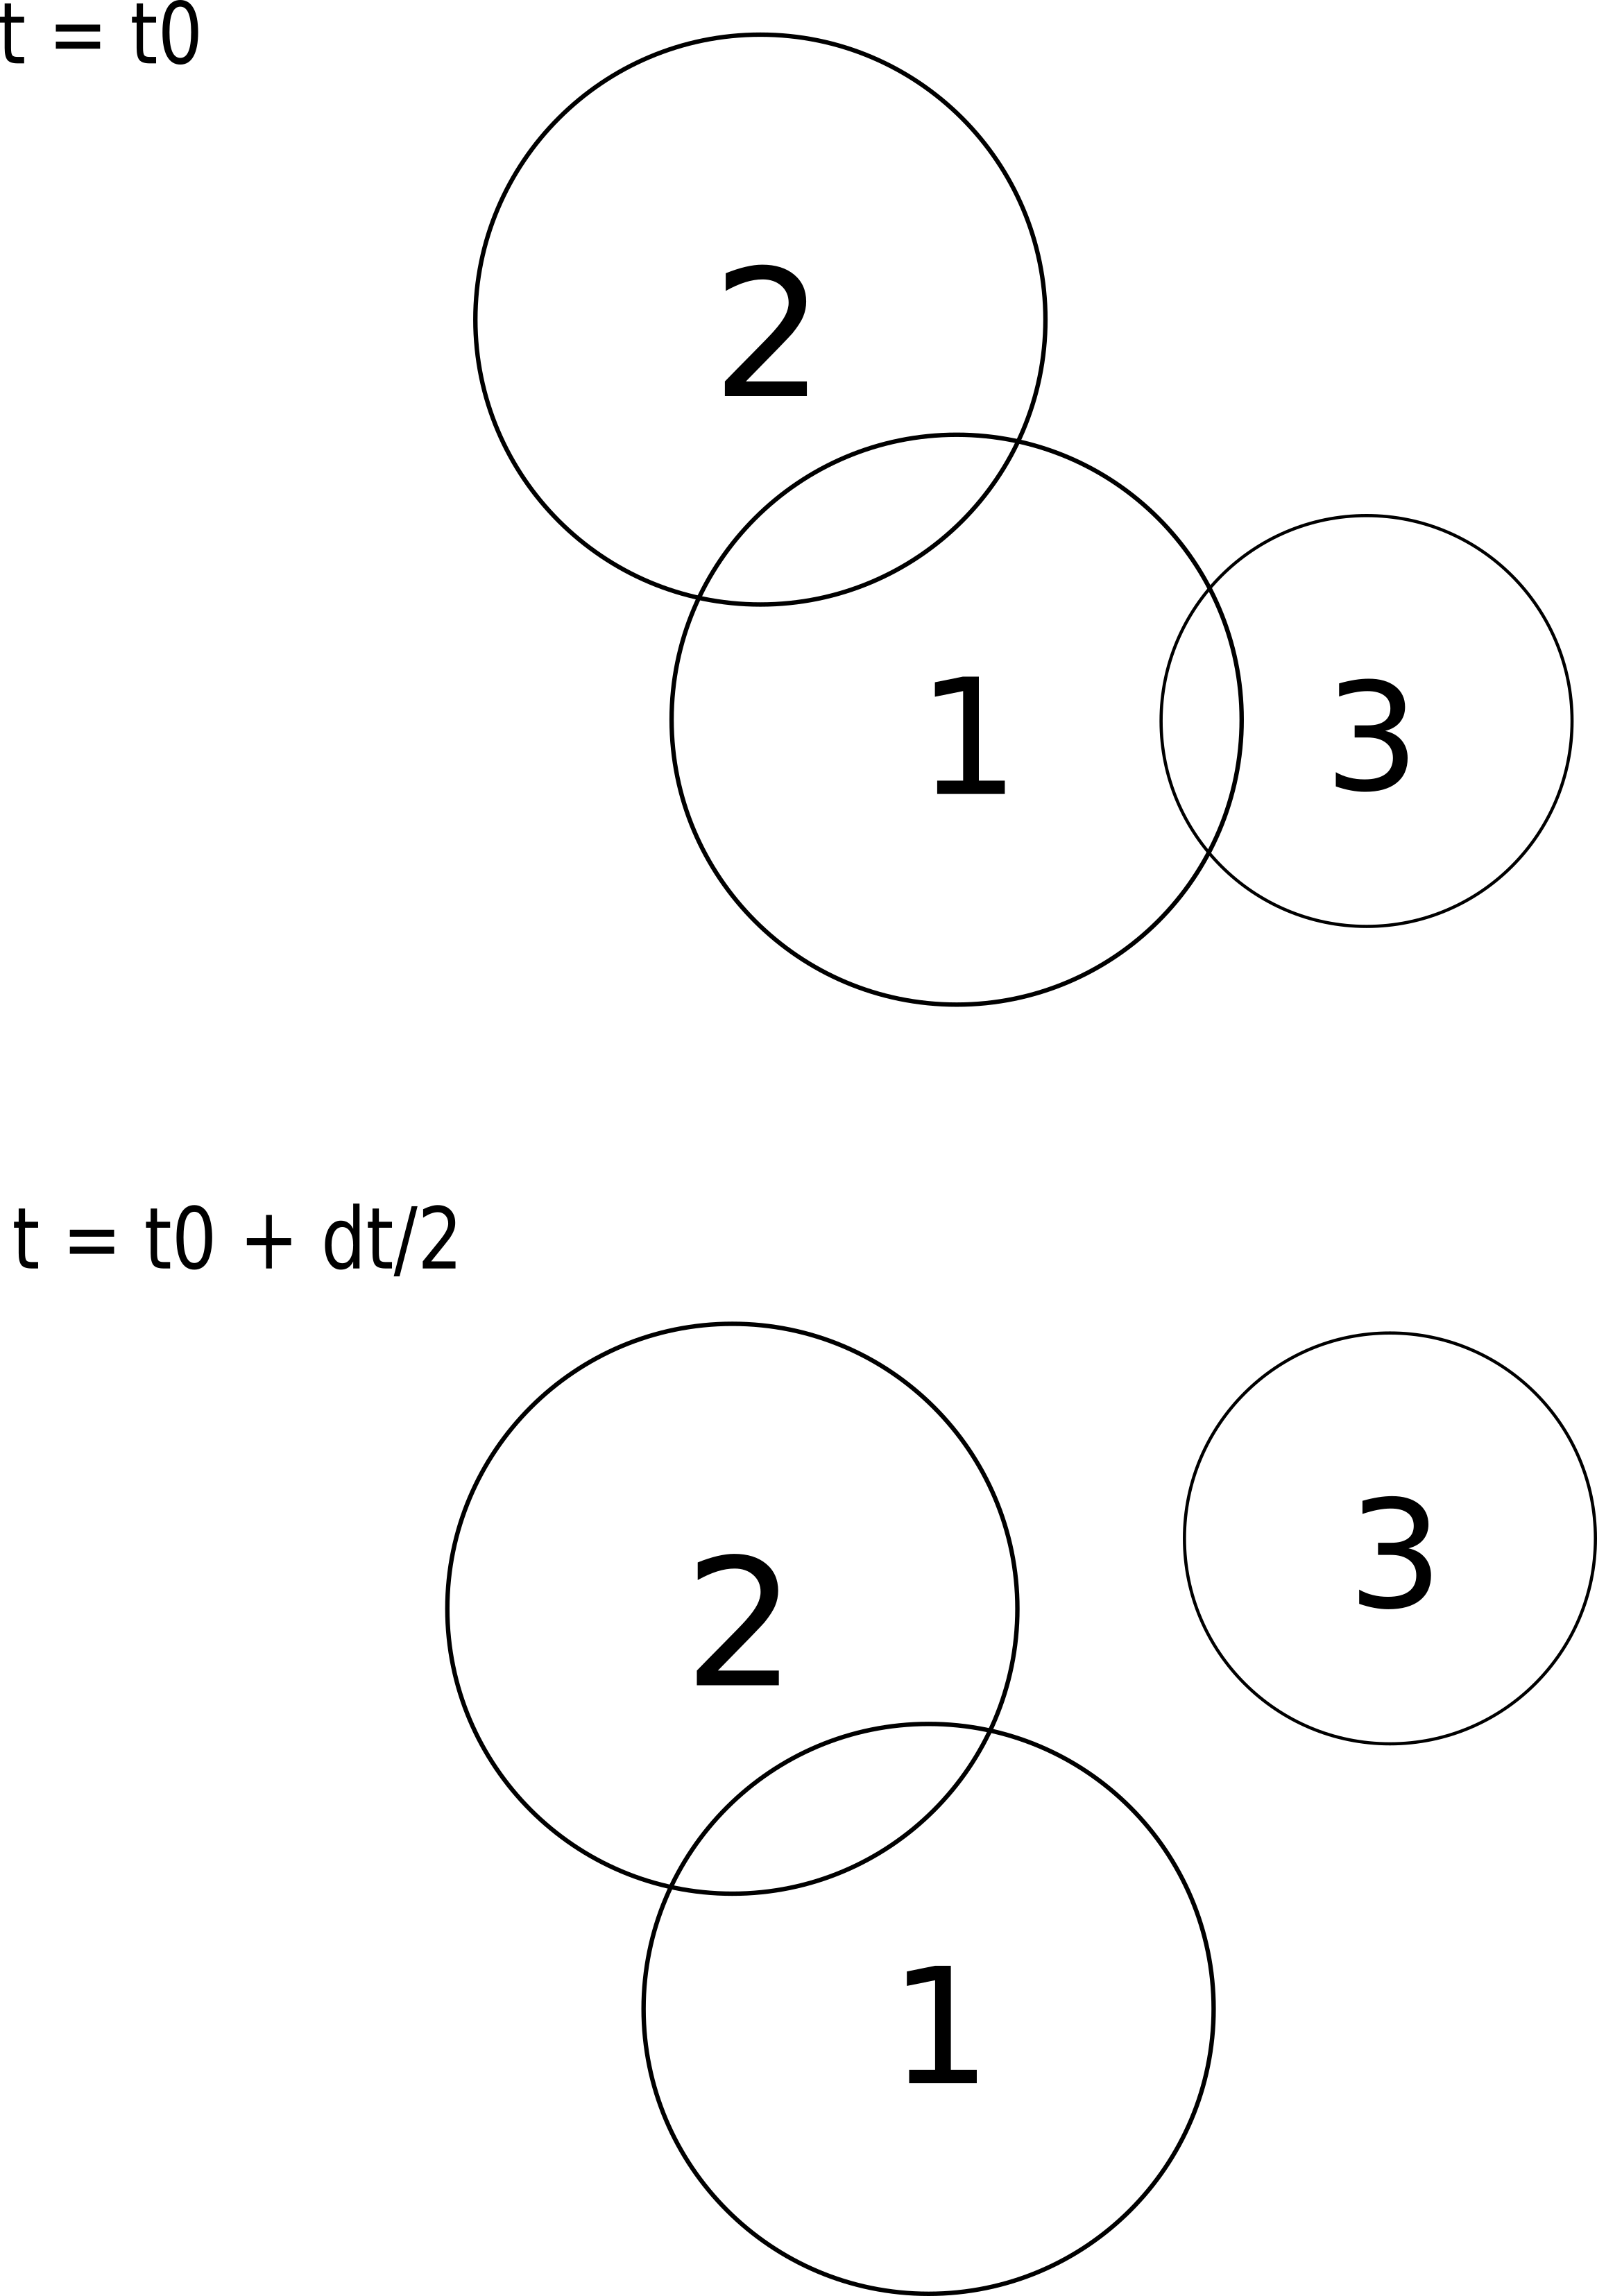
\includegraphics[scale=0.25]{dem_physics_figures/case2.png}
\caption{Particles at time t0, t0 + dt/2\label{fig:case2}}
\end{figure}

After \emph{stage1} particle 1 properties are

\begin{minted}[]{python}
        tng_x0 = [1.2, 2.1, 0., 0., 0.]
        tng_x = [1.5, 3.1, 0., 0., 0.]
	trk_idxs = [2, 3, -1, -1, -1]
	atng_x = [1.2, 2.1, 0., 0.]
\end{minted}

in \emph{compute\_accelerations} we see that particle 3 has left
the contact. In \emph{compute\_accelerations}, as particle 3 is checked for force
we get that it is not in contact. So we will not compute any force from
particle 3. Since we ignore particle 3 for force computation, the accelerations
of it are unchanged from time \(t0\). The properties of particle 1 after \emph{compute\_accelerations\_2}
would be

\begin{minted}[]{python}
	tng_x0 = [1.2, 2.1, 0., 0., 0.]
	tng_x = [1.5, 3.1, 0., 0., 0.]
	trk_idxs = [2, 3, -1, -1, -1]
	atng_x = [5.6, 2.1, 0., 0.]
\end{minted}

Please note that the \emph{atng\_x} of contact with particle 3 is not changed after
compute accelerations, this is due to particle 3 is no more in contact. But
rest of the contact accelerations are changed. In order to implement RK2
smoothly we will not remove the particle 3 at \(t0+dt/2\).

In stage 2

\begin{minted}[]{python}
	def stage2(self, ...):
	    # Code elided. Only tangential update is given
	    for i in range(0, num_ctcs):
		d_tng_x[i] = d_tng_x0[i] + dt * d_vt[i]
\end{minted}

Particle 3 tangential displacement will be incremented to time \(t0+dt\) by
using the velocity at time \(t0\) (since we didn't updated it at time
\(t0+dt/2\)).

After the time step we will check if particle 3 is still in overlap, if so
retain it else remove it.


\subsection{Case 3}
\label{sec:org2632dbe}
What if a particle comes into contact at a half time step? Here we simply add to
the tracking list and compute its acceleration at tme \(t0+dt/2\). In stage 2 using
the tangential acceleration at half time step, we will increment it to next time step.
This is done by

\begin{minted}[]{python}
	def stage2(self, ...):
	    # Code elided. Only tangential update is given
	    for i in range(0, num_ctcs):
		d_tng_x[i] = d_tng_x0[i] + dt * d_vt[i]
\end{minted}

Here the advantage is the tangential displacement at time \(t0\) is zero which
is taken care by \emph{tng\_x0}. By adding particle to the end automatically we are
assigning it a zero tangential displacement by default.


\bibliographystyle{unsrt}
\end{document}
\end{document}